\chapter{Kompression}\label{ch:Lektion}
\section{Einführung}

\subsection{Was ist Kompression?}

Der Begriff \enquote{Kompression} stammt --- wie viele andere Begriffe --- ursprünglich aus dem Latenischen (\textit{compressio} $=$ das Zusammendrücken, das Zusammenpressung, die Umarmung). Mit Kompression ist also häufig die ``Verkleinerung'', bzw. das ``Zusammendrücken'' von Daten gemeint, meist aus einem der folgenden Gründen:

\begin{enumerate}
	\item \textbf{Speicherplatz optimieren}: Angesichts des stets wachsenden Speicherbedarfs von Datenzentren sowie privaten Geräten wird es immer wichtiger, Dokumente zu ``komprimieren'', d.h., deren Grösse zu verringern, falls möglich (s. \cref{fig:compression-ex}).
\begin{figure}[H]
	\centering
	
\includegraphics[width=.6\textwidth]{GrundlagenInfo/04_Kompression/Figures/compression3}
	\caption{Beispiel einer Datei sowie deren Dateigrösse,  unkomprimiert (original) und komprimiert}
	\label{fig:compression-ex}
\end{figure}
\begin{figure}[H]
	\centering
	\raisebox{-0.5\height}{
\includegraphics[width=.2\textwidth]{GrundlagenInfo/04_Kompression/Figures/compression1}}
	\raisebox{-0.5\height}{$\rightarrow$}
	\raisebox{-0.5\height}{
\includegraphics[width=.25\textwidth]{GrundlagenInfo/04_Kompression/Figures/compression2}}
\end{figure}
	\item \textbf{Speicherplatz optimieren}: Häufig kann mit wenig Effort Speicherplatz optimiert werden, womit der Platzbedarf auf Speichermedien wie Festplatten verringert werden kann. Da Festplatten --- ähnlich einem Reisekoffer --- Kosten verursachen, will man den Speicherbedarf möglichst minimal halten (s. \cref{fig:speicherplatz-opt}).
\begin{figure}[H]
	\centering
	\raisebox{-0.5\height}{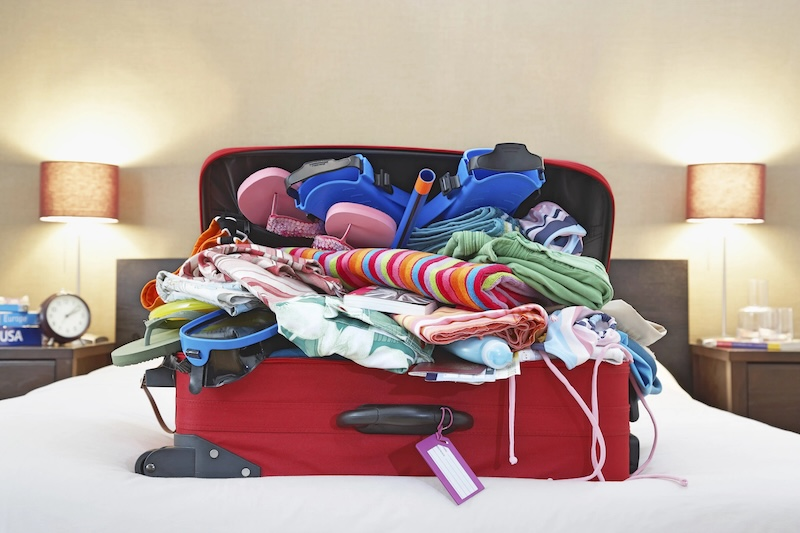
\includegraphics[width=.45\textwidth]{GrundlagenInfo/04_Kompression/Figures/messy_suitcase.jpg}}
	\raisebox{-0.5\height}{$\rightarrow$}
	\raisebox{-0.5\height}{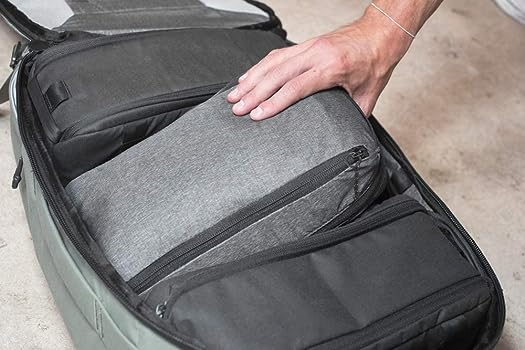
\includegraphics[width=.45\textwidth]{GrundlagenInfo/00_Programmieren/Figures/prog-packing-cubes}}
	\caption{Speicherplatz optimieren}
	\label{fig:speicherplatz-opt}
\end{figure}
	\item \textbf{Wartezeit verkürzen}: Computer und Geräte kommunizieren in Netzwerken, innerhalb welchen oftmals grosse Datenmengen übertragen werden müssen. Die Verbindungen zwischen den Geräten haben jedoch nur eine begrenzte Kapazität und werden daher häufig als \tib{Flaschenhälse} bezeichnet.
\begin{figure}[H]
\centering
\resizebox{!}{.5\height}{%
\begin{tikzpicture}
	\path[mindmap,concept color=black,text=white]
	node[concept] {Computer}
	[clockwise from=0]
	child[concept color=green!50!black] {
		node[concept] {Computer}
		[clockwise from=90]
		child { node[concept] {Computer} }
		child { node[concept] {Computer} }
		child { node[concept] {Computer} }
		child { node[concept] {Computer} }
	}  
	child[concept color=blue] {
		node[concept] {Computer}
		[clockwise from=-30]
		child { node[concept] {Computer} }
		child { node[concept] {Computer} }
	}
	child[concept color=red] { node[concept] {Computer} }
	child[concept color=orange] { node[concept] {Computer} };
\end{tikzpicture}}
\caption{Visualisierung von Computernetzwerken und deren \textit{Flaschenhälsen}}
\end{figure}
\end{enumerate}

Historischer Kontext
\begin{itemize}
	\item Leder und Stein: Teure Materialien
	\item Römische Zahlendarstellung: z.B. Zahl \textbf{999}
	\begin{center}
		\texttt{CCCCCCCCCXXXXXXXXXIIIIIIIII}\\
		$\downarrow$\\
		Erfindung der Ziffern D (500), L (50), V(5)\\
		$\downarrow$\\
		\texttt{DCCCCLXXXXVIIII} \\
		$\downarrow$\\
		Effizientere Schreibweise\\
		$\downarrow$\\
		IM
	\end{center}
\end{itemize}

\section{Verlustfreie vs. verlustbehaftete Kompression}
Einige Beispiele:
\begin{table}[H]
	\centering
	\begin{tabular}{c||c|c}
		\textbf{Anwendung} & \textbf{Verlustfrei} & \textbf{Verlustbehaftet} \\\midrule
		\textbf{Audio} & \texttt{.flac, .aac} & \texttt{.mp3}\\\hline
		\textbf{Dateien} & \texttt{.zip}, \texttt{.rar} & \texttt{-}\\\hline
		\textbf{Video} & \texttt{.raw} & \texttt{.mp4}, \texttt{.avi}, \texttt{.mov} \\\hline
		\textbf{Fotografie} & \texttt{.raw}, \texttt{.psd}, \texttt{.gif} & \texttt{.jpg}, \texttt{.png}\\\hline
		\textbf{Grafik} & \texttt{.svg}, \texttt{.pdf}
	\end{tabular}
\end{table}

\begin{figure}
	\centering
	\begin{subfigure}{.45\linewidth}
		\begin{tikzpicture}[boximg]
			\node[anchor=south west] (img) {
\includegraphics[width=\linewidth]{{GrundlagenInfo/04_Kompression/Figures/LeeLogo 300 dpi.jpg}}};
			\begin{scope}[x=(img.south east),y=(img.north west)]
				\node[draw,minimum height=.3cm,minimum width=.75cm] (B1) at (0.48,0.47) {};
			\end{scope}
		\end{tikzpicture}
		\caption{}
	\end{subfigure}\\[0.5\baselineskip]
	\begin{subfigure}{\linewidth}
		\begin{tikzpicture}[boximg]
			\node (img1) {
\includegraphics[width=0.9\linewidth]{GrundlagenInfo/04_Kompression/Figures/LeeLogo 300 dpi zoom}};
			\draw (img1.south west) rectangle (img1.north east);
		\end{tikzpicture}\hfill%
		\caption{}
	\end{subfigure}
	\begin{tikzpicture}[overlay,boximg]
		\draw (B1) -- (img1);
	\end{tikzpicture}
	\caption{\texttt{LeeLogo\textbf{.jpg} (48 KB, 300 dots per inch)}}
\end{figure}


		
\section{Kompressionsalgorithmen}

\begin{myexercise}
Was könnte folgende Sequenz bedeuten?
\begin{center}
WENN \emoji{blush} HINTER \emoji{blush} $\triangle$, $\triangle$ EINIGE \emoji{blush} ANDEREN \emoji{blush} NACH.
\end{center}
\begin{myanswer}
Mehrere Bedeutungen sind möglich, zum Beispiel:
\begin{center}
WENN GRIECHEN HINTER GRIECHEN RENNEN, RENNEN EINIGE GRIECHEN ANDEREN GRIECHEN NACH.
\end{center}
\end{myanswer}
\end{myexercise}

Wie können wir folgenden Text effizient Kodieren?

\begin{center}
AACABAAACBACAACADAAD
\end{center}

\begin{table}[H]
\centering
	\begin{tabular}{c|c|c|c|c}
		\textbf{Buchstabe} & \textbf{A} & \textbf{B} & \textbf{C} & \textbf{D} \\\midrule\midrule
		Häufigkeit & 12 &  2 & 4 & 2 \\\hline
		Relative Häufigkeit & 60\% & 10\% & 20\% & 10\% \\\hline
		``Naive'' Kodierung: & 00 & 01 & 10 & 11 \\\hline
		``Effiziente'' Kodierung: & 0 & 110  & 10&  111\\
	\end{tabular}
\end{table}
\begin{itemize}
	\item ``Naive'' Codierung (40 Zeichen):\\ \texttt{0000100001000000100100100000100011000011} 
	\item ``Effiziente'' Codierung (32 Zeichen, -20\% Ersparnis):\\ \texttt{0010110000101100100010011100111}\\

\end{itemize}

Beide Codierungen sind \textbf{präfixfrei}: Kein Codewort ist Anfangsstück (Präfix) eines anderen Codeworts

\begin{table}[H]
	\centering
		\begin{tabular}{c|c|c|c|c}
		\textbf{Buchstabe} & \textbf{A} & \textbf{B} & \textbf{C} & \textbf{D} \\\midrule\midrule
		Relative Häufigkeit & 60\% & 10\% & 20\% & 10\% \\\hline
		``Effiziente'' Kodierung: & 0 & 110  & 10&  111\\
	\end{tabular}
\end{table}
\begin{figure}[H]
	\centering
	\begin{tikzpicture}
		[-,>=stealth',level distance=15mm,
		level 1/.style={sibling distance=60mm},
		level 2/.style={sibling distance=30mm},
		level 3/.style={sibling distance=15mm},
		level 4/.style={sibling distance=15mm}, leaf/.style={circle, draw}, label/.style={red},edge from parent path={(\tikzparentnode.south) -- (\tikzchildnode)}] 
		
		
		\usetikzlibrary{shapes}
		\tikzstyle{c} = [draw, shape=circle]
		\tikzstyle{n} = [text width=1cm,align=center]
		\tikzstyle{r} = [text=red]
		
		\node[]{}[edge from parent]
		child {node[n] {A\\ \textcolor{red}{0}}
			edge from parent coordinate (ea);
		}
		child {node[]{}
			child {node[text width=1cm,align=center]{C\\ \textcolor{red}{10}}
				edge from parent coordinate (e25);
			}
			child {node[]{}
				child{node[n]{B\\ \textcolor{red}{110}}
					edge from parent coordinate (e14);
				}
				child{node[n]{D \\ \textcolor{red}{111}}
					edge from parent coordinate (e16);
				}
				edge from parent coordinate (e30);
			}
			edge from parent coordinate (e55);
		};
		% code labels
		\node[r] at([yshift=2mm]ea)  {0};
		\node[r] at([yshift=2mm]e55) {1};
		\node[r] at([xshift=-2mm,yshift=2mm]e25) {0};
		\node[r] at([xshift=2mm,yshift=2mm]e30) {1};
		\node[r] at([xshift=-2mm,yshift=1mm]e14) {0};
		\node[r] at([xshift=2mm,yshift=1mm]e16) {1};
	\end{tikzpicture}
\end{figure}

\subsection{Top-Down-Ansatz: Maximale Balance}
\textbf{Idee}: Summe der Buchstabenhäufigkeiten im linken und rechten Teilbaum ausbalancieren

\begin{table}[H]
	\centering
	\begin{tabular}{c|c|c|c|c|c|c}
		\textbf{Buchstabe} & \textbf{A} & \textbf{B} & \textbf{C} & \textbf{D}& \textbf{E}& \textbf{F} \\\midrule\midrule
		Relative Häufigkeit & 25\% & 25\% & 13\% & 13\%& 12\%& 12\%
	\end{tabular}
	\caption{Beispiel-Häufigkeiten von Buchstaben}
	\label{table:ex-topdown}
\end{table}

\begin{figure}[H]
\centering
\begin{subfigure}{.55\textwidth}
\centering
\begin{tikzpicture}
	[-,>=stealth',
	level distance=18mm,
	level 1/.style={sibling distance=60mm},
	level 2/.style={sibling distance=30mm},
	level 3/.style={sibling distance=15mm},
	level 4/.style={sibling distance=8mm},
	leaf/.style={circle, draw},
	label/.style={red},
	edge from parent path={(\tikzparentnode.south) -- (\tikzchildnode)}] 
	
	
	\usetikzlibrary{shapes}
	\tikzstyle{n} = [text width=1cm,align=center]
	\tikzstyle{r} = [text=red]
	
	\node[n]{\textcolor{BlueGreen}{A,B,C,D,E,F}\\ 100\%}[edge from parent]
	child {node[n] {\textcolor{BlueGreen}{A,B}\\ 50\%}
		edge from parent node[left,r]{0};
	}
	child {node[n]{\textcolor{BlueGreen}{C,D,E,F}\\ 50\%}
		edge from parent node[r,right]{1};
	};
\end{tikzpicture}
\caption{Schritt 1}
\end{subfigure}
\begin{subfigure}{.55\textwidth}
\centering
\begin{tikzpicture}
	[-,>=stealth',
	level distance=18mm,
	level 1/.style={sibling distance=60mm},
	level 2/.style={sibling distance=30mm},
	level 3/.style={sibling distance=15mm},
	level 4/.style={sibling distance=8mm},
	leaf/.style={circle, draw},
	label/.style={red},
	edge from parent path={(\tikzparentnode.south) -- (\tikzchildnode)}] 
	
	
	\usetikzlibrary{shapes}
	\tikzstyle{n} = [text width=1cm,align=center]
	\tikzstyle{r} = [text=red]
	
	\node[n]{\textcolor{BlueGreen}{A,B,C,D,E,F}\\ 100\%}[edge from parent]
	child {node[n] {\textcolor{BlueGreen}{A,B}\\ 50\%}
			child {node[n] {\textcolor{BlueGreen}{A}\\ 25\%\\\textcolor{red}{00}}
				edge from parent[] node[left,r]{0};
			}
			child {node[n] {\textcolor{BlueGreen}{B}\\ 25\%\\\textcolor{red}{01}}
				edge from parent[] node[r,right]{1};
			}
		edge from parent node[left,r]{0};
	}
	child {node[n]{\textcolor{BlueGreen}{C,D,E,F}\\ 50\%}
		edge from parent node[r,right]{1};
	};
\end{tikzpicture}
\caption{Schritt 2}
\end{subfigure}
\begin{subfigure}{.55\textwidth}
\centering
\begin{tikzpicture}
	[-,>=stealth',
	level distance=18mm,
	level 1/.style={sibling distance=60mm},
	level 2/.style={sibling distance=30mm},
	level 3/.style={sibling distance=15mm},
	level 4/.style={sibling distance=8mm},
	leaf/.style={circle, draw},
	label/.style={red},
	edge from parent path={(\tikzparentnode.south) -- (\tikzchildnode)}] 
	
	
	\usetikzlibrary{shapes}
	\tikzstyle{n} = [text width=1cm,align=center]
	\tikzstyle{r} = [text=red]
	
	\node[n]{\textcolor{BlueGreen}{A,B,C,D,E,F}\\ 100\%}[edge from parent]
	child {node[n] {\textcolor{BlueGreen}{A,B}\\ 50\%}
			child {node[n] {\textcolor{BlueGreen}{A}\\ 25\%\\\textcolor{red}{00}}
				edge from parent[] node[left,r]{0};
			}
			child {node[n] {\textcolor{BlueGreen}{B}\\ 25\%\\\textcolor{red}{01}}
				edge from parent[] node[r,right]{1};
			}
		edge from parent node[left,r]{0};
	}
	child {node[n]{\textcolor{BlueGreen}{C,D,E,F}\\ 50\%}
			child {node[n] {\textcolor{BlueGreen}{C,E}\\ 25\%}
				edge from parent[] node[left,r]{0};
			}
			child {node[n] {\textcolor{BlueGreen}{D,F}\\ 25\%}
				edge from parent[] node[r,right]{1};
			}
		edge from parent node[r,right]{1};
	};
\end{tikzpicture}
\caption{Schritt 3}
\end{subfigure}

\begin{subfigure}{.5\textwidth}
\centering
\begin{tikzpicture}
	[-,>=stealth',
	level distance=18mm,
	level 1/.style={sibling distance=60mm},
	level 2/.style={sibling distance=30mm},
	level 3/.style={sibling distance=15mm},
	level 4/.style={sibling distance=8mm},
	leaf/.style={circle, draw},
	label/.style={red},
	edge from parent path={(\tikzparentnode.south) -- (\tikzchildnode)}] 
	
	
	\usetikzlibrary{shapes}
	\tikzstyle{n} = [text width=1cm,align=center]
	\tikzstyle{r} = [text=red]
	
	\node[n]{\textcolor{BlueGreen}{A,B,C,D,E,F}\\ 100\%}[edge from parent]
	child {node[n] {\textcolor{BlueGreen}{A,B}\\ 50\%}
		child {node[n] {\textcolor{BlueGreen}{A}\\ 25\%\\\textcolor{red}{00}}
			edge from parent[] node[left,r]{0};
		}
		child {node[n] {\textcolor{BlueGreen}{B}\\ 25\%\\\textcolor{red}{01}}
			edge from parent[] node[r,right]{1};
		}
		edge from parent node[left,r]{0};
	}
	child {node[n]{\textcolor{BlueGreen}{C,D,E,F}\\ 50\%}
		child {node[n] {\textcolor{BlueGreen}{C,E}\\ 25\%}
			child {node[n] {\textcolor{BlueGreen}{C}\\ 13\%\\\textcolor{red}{100}}
				edge from parent[] node[left,r]{0};
			}
			child {node[n] {\textcolor{BlueGreen}{E}\\ 12\%\\\textcolor{red}{101}}
				edge from parent[] node[r,right]{1};
			}
			edge from parent[] node[left,r]{0};
		}
		child {node[n] {\textcolor{BlueGreen}{D,F}\\ 25\%}
			child {node[n] {\textcolor{BlueGreen}{D}\\ 13\%\\\textcolor{red}{110}}
				edge from parent[] node[left,r]{0};
			}
			child {node[n] {\textcolor{BlueGreen}{F}\\ 12\%\\\textcolor{red}{111}}
				edge from parent[] node[r,right]{1};
			}
			edge from parent[] node[r,right]{1};
		}
		edge from parent node[r,right]{1};
	};
\end{tikzpicture}
\caption{Schritt 4}
\end{subfigure}
\caption{Schritt-für-Schritt-Erstellung des Baumdiagramms für \cref{table:ex-topdown} mit dem \tib{Top-Down}-Ansatz.}
\end{figure}

\begin{myexercise}
\textbf{Problem}: Was passiert bei folgender Verteilung?
		\begin{table}[H]
			\centering
			\begin{tabular}{c|c|c|c|c|c|c}
				\textbf{Buchstabe} & \textbf{A} & \textbf{B} & \textbf{C} & \textbf{D}& \textbf{E}& \textbf{F} \\\midrule\midrule
				Relative Häufigkeit &.55\% & 1\% & 25\% & 8\%& 9\%& 8\%
			\end{tabular}
	\end{table}


	\begin{myanswer}
	\begin{figure}[H]
	\centering
	\begin{tikzpicture}
				[-,>=stealth',
				level distance=15mm,
				level 1/.style={sibling distance=60mm},
				level 2/.style={sibling distance=30mm},
				level 3/.style={sibling distance=15mm},
				level 4/.style={sibling distance=15mm},
				level 5/.style={sibling distance=15mm},
				leaf/.style={circle, draw},
				label/.style={red},
				edge from parent path={(\tikzparentnode.south) -- (\tikzchildnode)}] 
				
				
				\usetikzlibrary{shapes}
				\tikzstyle{n} = [text width=1cm,align=center]
				\tikzstyle{r} = [text=red]
				
				\node[n]{\textcolor{BlueGreen}{A,B,C,D,E,F}\\ 100\%}[edge from parent]
				child {node[n] {\textcolor{BlueGreen}{A,B}\\ 50\%}
					child {node[n] {\textcolor{BlueGreen}{A}\\.55\%\\\textcolor{red}{00}}
						edge from parent[] node[left,r]{0};
					}
					child {node[n, draw] {\textcolor{BlueGreen}{B}\\ 1\%\\\textcolor{red}{01}}
						edge from parent[] node[r,right]{1};
					}
					edge from parent node[left,r]{0};
				}
				child {node[n]{\textcolor{BlueGreen}{C,D,E,F}\\ 50\%}
					child {node[n] {\textcolor{BlueGreen}{C}\\ 25\%\\\textcolor{red}{10}}
						edge from parent[] node[left,r]{0};
					}
					child {node[n] {\textcolor{BlueGreen}{D,E,F}\\ 25\%}
						child {node[n] {\textcolor{BlueGreen}{D,E}\\ 17\%\\}
							child {node[n, draw] {\textcolor{BlueGreen}{D}\\ 8\%\\\textcolor{red}{1100}}
								edge from parent[] node[left,r]{0};
							}
							child {node[n, draw] {\textcolor{BlueGreen}{E}\\ 9\%\\\textcolor{red}{1101}}
								edge from parent[] node[right,r]{1};
							}
							edge from parent[] node[left,r]{0};
						}
						child {node[n, draw] {\textcolor{BlueGreen}{F}\\ 8\%\\\textcolor{red}{111}}
							edge from parent[] node[r,right]{1};
						}
						edge from parent[] node[r,right]{1};
					}
					edge from parent node[r,right]{1};
				};
			\end{tikzpicture}
	\end{figure}
	Wie wir sehen, wird der resultierende Baum nicht ausgeglichen: während der Buchstabe ``F'' (8\% Häufigkeit im Originaltext) beispielsweise mit ``111'' kodiert wird, wird der Buchstabe ``B'' (1 \% Häufigkeit im Originaltext) mit ``01'' kodiert, also mit einer kürzeren Bitfolge. Wie wir allerdings gesehen haben, sollten Buchstaben mit höherer Häufigkeit kürzer kodiert werden, da wir sie ja häufiger kodieren müssen und mit einer kürzeren Kodierungslänge somit insgesamt mehr Speicherplatz sparen.
\end{myanswer}
	
\end{myexercise}
\subsection{Bottom-Up-Ansatz: Huffmann-Kodierung}

Idee: 
\begin{itemize}
		\item Jeder Buchstabe wird als Graph mit einem Knoten (=Baum mit einem Blatt) betrachtet. Die Häufigkeit jedes Buchstabens wird neben dem Blatt notiert. Wir wollen nun die Buchstaben zu Teilbäumen verbinden, bis wir einen einzigen Baum haben.
		\begin{figure}[H]
			\centering
			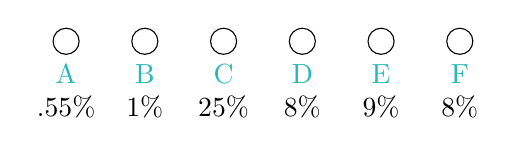
\begin{tikzpicture}
				\tikzstyle{n} = [text width=1cm,align=center, draw, shape=circle]
				\node[circle,draw, label={[align=center]below:\textcolor{BlueGreen}{A}\\.55\%}, ](a){};
				\node[circle,draw, label={[align=center]below:\textcolor{BlueGreen}{B}\\ 1\%}, right of=a](b){};
				\node[circle,draw, label={[align=center]below:\textcolor{BlueGreen}{C}\\ 25\%}, right of=b](c){};
				\node[circle,draw, label={[align=center]below:\textcolor{BlueGreen}{D}\\ 8\%}, right of=c](d){};
				\node[circle,draw, label={[align=center]below:\textcolor{BlueGreen}{E}\\ 9\%}, right of=d](e){};
				\node[circle,draw, label={[align=center]below:\textcolor{BlueGreen}{F}\\ 8\%}, right of=e](f){};
			\end{tikzpicture}
			\caption{Beispiel-Häufigkeiten von Buchstaben}
			\label{fig:exFreqHuffmann}
		\end{figure}
		\item In einer Schleife: Wir schauen alle isolierten Blätter und Wurzeln von Teilbäumen an. Diejenigen  Knoten, die die kleinste (gemeinsame) Prozentzahl enthalten werden miteinander verbunden. Die neue Wurzel wird markiert mit dem Prozentsatz beider Knoten.
		\begin{figure}[H]
			\centering
			\begin{tikzpicture}[-,>=stealth',
				level distance=12mm,
				level 1/.style={sibling distance=15mm},
				level 2/.style={sibling distance=30mm},
				level 3/.style={sibling distance=15mm},
				level 4/.style={sibling distance=15mm},
				level 5/.style={sibling distance=15mm},
				leaf/.style={circle, draw},
				edge from parent path={(\tikzparentnode.south) -- (\tikzchildnode)}] 
				
				
				\usetikzlibrary{shapes}
				\tikzstyle{n} = [text width=1cm,align=center]
				\tikzstyle{r} = [text=red]
				
				\node[n]{\textcolor{BlueGreen}{B,D}\\ 9\%}[edge from parent]
				child {node[n] {\textcolor{BlueGreen}{B}\\ 1\%}
					edge from parent node[left,r]{};
				}
				child {node[n]{\textcolor{BlueGreen}{D}\\ 8\%}
					edge from parent node[r,right]{};
				};
			\end{tikzpicture}
			\caption{Erster Schritt im Huffmann-Kodierungs-Algorithmus}
		\end{figure}
		\item Falls mehrere Möglichkeiten mit gleicher relativer Häufigkeit existieren, nehmen wir den Teilbaum mit der geringsten Tiefe.
		\end{itemize}
\textbf{Welche Knoten werden als nächstes miteinander verbunden?}

\begin{figure}[H]
	\centering
	\begin{subfigure}{.55\textwidth}
	\begin{tikzpicture}[-,>=stealth',
		level distance=15mm,
		level 1/.style={sibling distance=15mm},
		level 2/.style={sibling distance=30mm},
		level 3/.style={sibling distance=15mm},
		level 4/.style={sibling distance=15mm},
		level 5/.style={sibling distance=15mm},
		leaf/.style={circle, draw},
		edge from parent path={(\tikzparentnode.south) -- (\tikzchildnode)}] 
		
		
		\usetikzlibrary{shapes}
		\tikzstyle{n} = [text width=1cm,align=center]
		\tikzstyle{r} = [text=red]

		\node(bd)[n]{\textcolor{BlueGreen}{B,D}\\ 9\%}[edge from parent]
		child {node(b)[n] {\textcolor{BlueGreen}{B}\\ 1\%}
			edge from parent node[left,r]{} ;
		}
		child {node[n]{\textcolor{BlueGreen}{D}\\ 8\%}
			edge from parent node[r,right]{};
		};
		\node(ef)[n, left of=bd,xshift=-15mm]{\textcolor{BlueGreen}{E,F}\\ 17\%}[edge from parent]
		child {node(f)[n] {\textcolor{BlueGreen}{F}\\ 8\%}
			edge from parent node[left,r]{} ;
		}
		child {node[n]{\textcolor{BlueGreen}{E}\\ 9\%}
			edge from parent node[r,right]{};
		};
		\node[n, left of=f](c){\textcolor{BlueGreen}{C}\\ 25\%};
		\node[n, left of=c](a){\textcolor{BlueGreen}{A}\\.55\%};
	\end{tikzpicture}
	\caption{Schritt 1}
	\end{subfigure}
	\begin{subfigure}{.55\textwidth}
	\begin{tikzpicture}[-,>=stealth',
			level distance=15mm,
			level 1/.style={sibling distance=30mm},
			level 2/.style={sibling distance=15mm},
			level 3/.style={sibling distance=15mm},
			level 4/.style={sibling distance=15mm},
			level 5/.style={sibling distance=15mm},
			leaf/.style={circle, draw},
			edge from parent path={(\tikzparentnode.south) -- (\tikzchildnode)}] 
			
			\usetikzlibrary{shapes}
			\tikzstyle{n} = [text width=1cm,align=center]
			\tikzstyle{r} = [text=red]
			
			\node(febd)[n]{\textcolor{BlueGreen}{F,E,B,D}\\ 26\%}[edge from parent]
				child{node(ef)[n]{\textcolor{BlueGreen}{E,F}\\ 17\%}
					child {node(f)[n] {\textcolor{BlueGreen}{F}\\ 8\%}
						edge from parent node[left,r]{} ;
					}
					child {node[n]{\textcolor{BlueGreen}{E}\\ 9\%}
						edge from parent node[r,right]{};
					}
					edge from parent node[r,right]{};
				}
				child{node(bd)[n]{\textcolor{BlueGreen}{B,D}\\ 9\%}
					child {node(b)[n] {\textcolor{BlueGreen}{B}\\ 1\%}
						edge from parent node[left,r]{} ;
					}
					child {node[n]{\textcolor{BlueGreen}{D}\\ 8\%}
						edge from parent node[r,right]{};
					}
					edge from parent node[r,left]{};
				};
			\node[n, left of=f](c){\textcolor{BlueGreen}{C}\\ 25\%};
			\node[n, left of=c](a){\textcolor{BlueGreen}{A}\\.55\%};
		\end{tikzpicture}
		\caption{Schritt 2}
	\end{subfigure}
	\begin{subfigure}{.55\textwidth}
	\begin{tikzpicture}[-,>=stealth',
			level distance=15mm,
			level 1/.style={sibling distance=60mm},
			level 2/.style={sibling distance=30mm},
			level 3/.style={sibling distance=30mm},
			level 4/.style={sibling distance=15mm},
			level 5/.style={sibling distance=15mm},
			leaf/.style={circle, draw},
			edge from parent path={(\tikzparentnode.south) -- (\tikzchildnode)}] 
			
			\usetikzlibrary{shapes}
			\tikzstyle{n} = [text width=1cm,align=center]
			\tikzstyle{r} = [text=red]
			
			\node(acebd)[n]{\textcolor{BlueGreen}{A,C,F,E,B,D}\\ 100\%}[edge from parent]
			child{node(a)[n]{\textcolor{BlueGreen}{A}\\.55\%}
				edge from parent node[left,r]{} ;
			}
			child{node(cfebd)[n]{\textcolor{BlueGreen}{C,F,E,B,D}\\ 51\%}
				child{node(c)[n]{\textcolor{BlueGreen}{C}\\ 25\%}
					edge from parent node[left,r]{} ;
					}
				child{node(febd)[n]{\textcolor{BlueGreen}{F,E,B,D}\\ 26\%}
					child{node(ef)[n]{\textcolor{BlueGreen}{E,F}\\ 17\%}
						child {node(f)[n] {\textcolor{BlueGreen}{F}\\ 8\%}
							edge from parent node[left,r]{} ;
						}
						child {node[n]{\textcolor{BlueGreen}{E}\\ 9\%}
							edge from parent node[r,right]{};
						}
						edge from parent node[r,right]{};
					}
					child{node(bd)[n]{\textcolor{BlueGreen}{B,D}\\ 9\%}
						child {node(b)[n] {\textcolor{BlueGreen}{B}\\ 1\%}
							edge from parent node[left,r]{} ;
						}
						child {node[n]{\textcolor{BlueGreen}{D}\\ 8\%}
							edge from parent node[r,right]{};
						}
						edge from parent node[r,left]{};
					}
				edge from parent node[right,r]{};
				}
				edge from parent node[right,r]{};
			};		
		\end{tikzpicture}
		\caption{Schritt 3}
	\end{subfigure}
	\begin{subfigure}{.55\textwidth}
	\begin{tikzpicture}[-,>=stealth',
			level distance=15mm,
			level 1/.style={sibling distance=60mm},
			level 2/.style={sibling distance=30mm},
			level 3/.style={sibling distance=30mm},
			level 4/.style={sibling distance=15mm},
			level 5/.style={sibling distance=15mm},
			leaf/.style={circle, draw},
			edge from parent path={(\tikzparentnode.south) -- (\tikzchildnode)}] 
			
			\usetikzlibrary{shapes}
			\tikzstyle{n} = [text width=1cm,align=center]
			\tikzstyle{r} = [text=red]
			
			\node(acebd)[n]{\textcolor{BlueGreen}{A,C,F,E,B,D}\\ 100\%}[edge from parent]
			child{node(a)[n]{\textcolor{BlueGreen}{A}\\.55\%\\\textcolor{red}{0}}
				edge from parent node[left,r]{0} ;
			}
			child{node(cfebd)[n]{\textcolor{BlueGreen}{C,F,E,B,D}\\ 51\%}
				child{node(c)[n]{\textcolor{BlueGreen}{C}\\ 25\%\\\textcolor{red}{10}}
					edge from parent node[left,r]{0} ;
				}
				child{node(febd)[n]{\textcolor{BlueGreen}{F,E,B,D}\\ 26\%}
					child{node(ef)[n]{\textcolor{BlueGreen}{E,F}\\ 17\%}
						child {node(f)[n] {\textcolor{BlueGreen}{F}\\ 8\%\\\textcolor{red}{1100}}
							edge from parent node[left,r]{0} ;
						}
						child {node[n]{\textcolor{BlueGreen}{E}\\ 9\%\\\textcolor{red}{1101}}
							edge from parent node[r,right]{1};
						}
						edge from parent node[r,left]{0};
					}
					child{node(bd)[n]{\textcolor{BlueGreen}{B,D}\\ 9\%}
						child {node(b)[n] {\textcolor{BlueGreen}{B}\\ 1\%\\\textcolor{red}{1110}}
							edge from parent node[left,r]{0} ;
						}
						child {node[n]{\textcolor{BlueGreen}{D}\\ 8\%\\\textcolor{red}{1111}}
							edge from parent node[r,right]{1};
						}
						edge from parent node[r,right]{1};
					}
					edge from parent node[right,r]{1};
				}
				edge from parent node[right,r]{1};
			};		
		\end{tikzpicture}
		\caption{Schritt 4}
	\end{subfigure}
	\caption{Schritt-für-Schritt-Erstellung des Baumdiagramms für \cref{fig:exFreqHuffmann} mit der \tib{Huffmann}-Kodierung}
\end{figure}

\begin{myexercise}
Weshalb haben wir in Schritt 2 einen Baum \{\textcolor{BlueGreen}{E,F}\} statt \{\textcolor{BlueGreen}{F,B,D}\} gemacht?
\end{myexercise}	
		
Als Fazit kann folgendes festgehalten werden:
\begin{itemize}
	\item Strategie der \textbf{Maximale Balance}: \textit{top-down}-Ansatz (von Wurzel zu Blättern), kann zu suboptimalen Kodierungen führen
	\item \textbf{Huffman-Kodierung}: \textit{bottom-up}-Ansatz (von Blättern zur Wurzel), garantiert bestmögliche Kodierungslänge für alle Buchstaben
\end{itemize}

\begin{myexercise}
Komprimieren Sie das Wort ``Allemal'' mit der Huffman-Kodierung.
\end{myexercise}

\begin{myexercise}
	Klicken Sie auf \href{https://cmps-people.ok.ubc.ca/ylucet/DS/Huffman.html}{diesen Link}, um Huffman-Bäume Schritt-für-Schritt zu visualisieren
\end{myexercise}